\subsubsection{Annulus composition}
\label{sec:annulus-composition}

Let $\annradii \in [0, 1]^{\diam \times \diam}$ be a matrix containing the distances (radii) of each pixel from the middle of the annulus matrix of the size $\diam \times \diam$. If $\diam = 1$,
\begin{equation}
    \annradii = 
    \begin{pmatrix}
        0
    \end{pmatrix}.
\end{equation}
Otherwise, for $i, j \in \{ 0, 1, \cdots,  \diam-1 \}$,
\begin{equation}
    \annradii_{i, j} = \left\| 
        \left(
            -\frac{\diamdg}{2} + \frac{\diamdg}{\diam - 1} i, 
            -\frac{\diamdg}{2} + \frac{\diamdg}{\diam - 1} j 
        \right) 
    \right\|,
\end{equation}
where $\diamdg \in \mathbb{R}_+$ is the physical diameter of the annulus.

Let $\annmatrix \in [0, 1]^{\diam \times \diam}$ be the pixel luminance matrix of the annulus. Then, for $i, j \in \{ 0, 1, \cdots,  \diam-1 \}$,
\begin{equation}
    \annmatrix_{i, j} = \vlum \cdot
    \begin{cases}
        \cos(2 \pi \annradii_{i, j} \spatfreq + \pi) 
        &\text{ if } \annradii_{i, j} \leq \frac{\diamdg}{2} \\
        1 
        &\text{ otherwise}
    \end{cases},
    \label{eq:grating}
\end{equation}
where $\vlum \in [0, 1]$ is luminance of the void (the area uncovered by the annulus) and $\spatfreq \in \mathbb{R}_+$ is the spatial frequency.
An example of the resulting luminance matrix' greyscale heat map is visualized in Figure \ref{fig:grating-example}.

\begin{figure}[!htp]
    \centering
    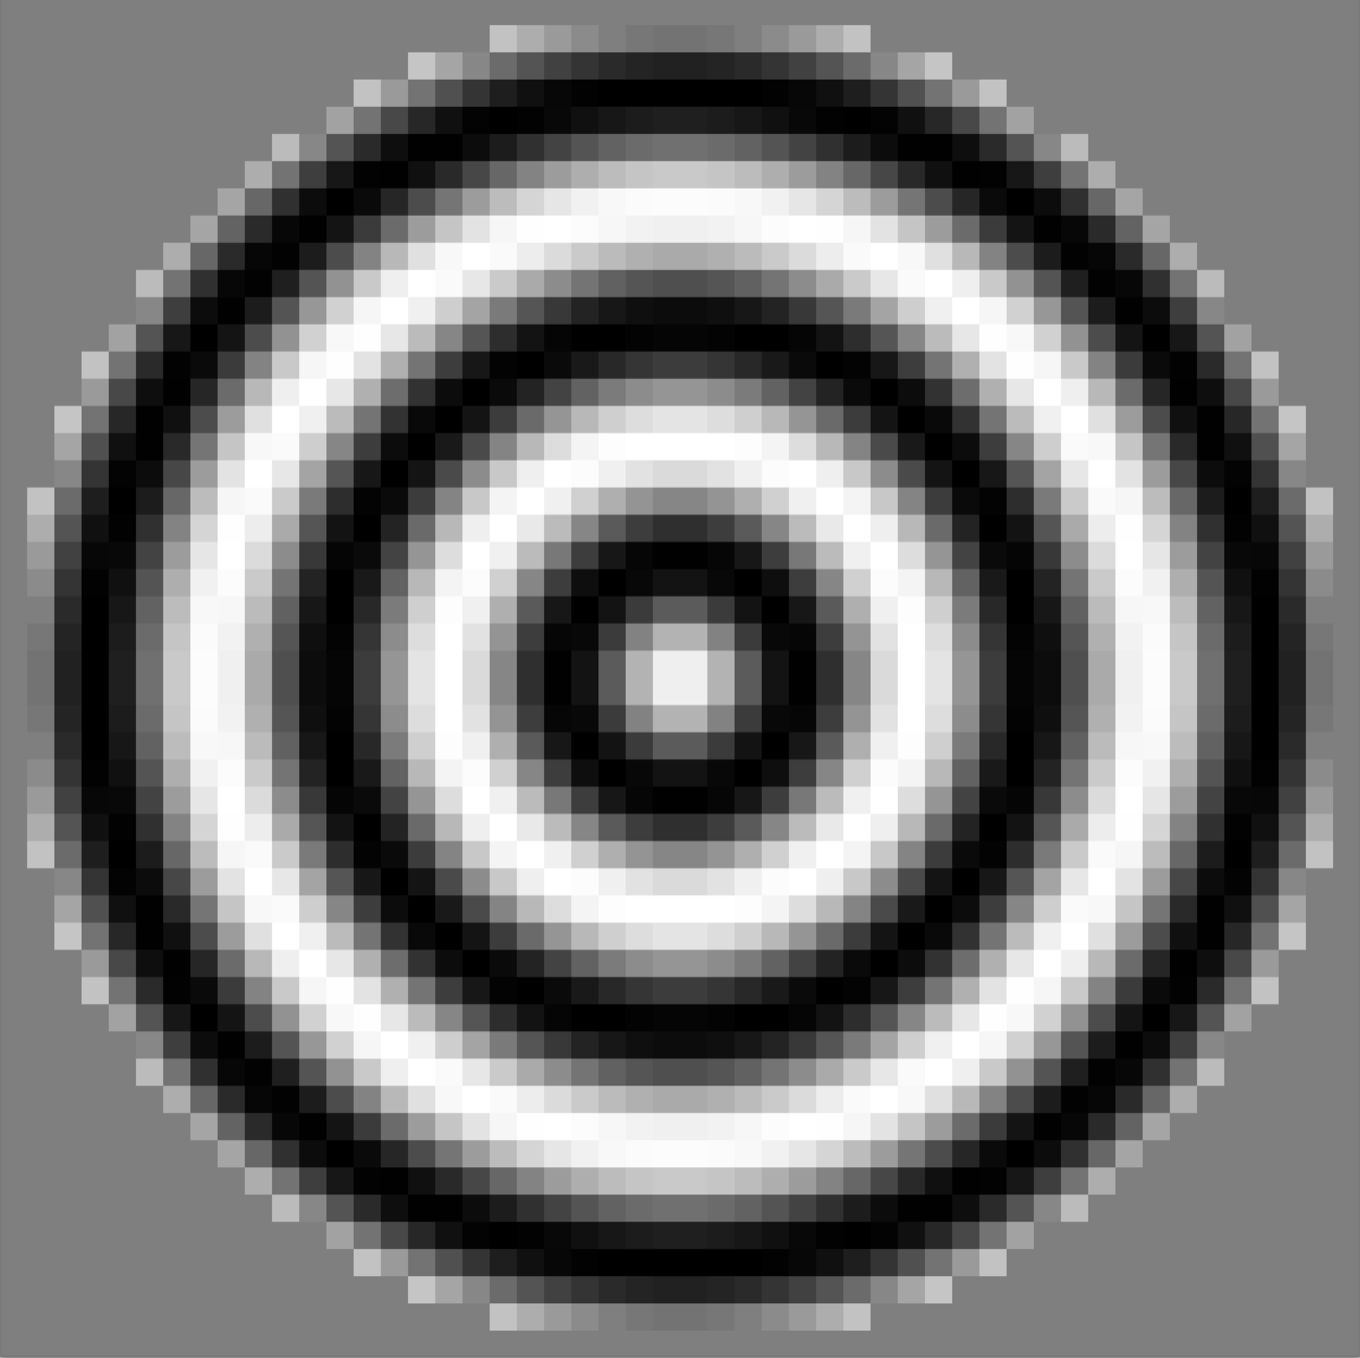
\includegraphics[width=0.2\textwidth]{assets/images/grating.png}
    \caption[Grating annulus]{An example of the annulus grating with maximal contrast and $\spatfreq = 5.7 \text{ cycles}/\circ, \vlum = 0.5, \diamdg = 0.7^\circ, \diam = 50$.}
    \label{fig:grating-example}
\end{figure}